
% {{{ preamble

%\documentclass[10pt,letterpaper]{article}
\documentclass{article}
%\documentclass[twocolumn]{article}
%\documentclass[12pt]{report}

\usepackage{url}
\usepackage{hyperref}
\usepackage{graphicx}
\usepackage{multicol}
\usepackage{tikz}
\usepackage{tikz-timing}
\usepackage{nonfloat}
\usepackage{amsmath}
\usepackage{mathtools}
\usepackage{fancyvrb}

\usepackage{listings}
\lstset{numbers=left,
		language=C,
		tabsize=4,
		showstringspaces=false,  % don't show the space character
		%basicstyle=\footnotesize,
		basicstyle=\normalsize,
		captionpos=b,
		xleftmargin=0.3in}

\usepackage{sectsty}  % \sectionfont
\sectionfont{\normalsize}
\subsectionfont{\normalsize}

%\usepackage{fancyhdr}
%\pagestyle{fancy}
%\fancyhf{}
%\renewcommand{\headrulewidth}{0pt}
%\renewcommand{\footrulewidth}{0pt}
%\rhead{\thepage}

\usepackage{vmargin}  % make the margins a bit smaller
%\setmarginsrb{1.0in}{1.0in}{1.0in}{1.0in}{0in}{0.4in}{0.0in}{0.40in}
\setmarginsrb{1.0in}{1.0in}{1.0in}{1.0in}{0in}{0.25in}{0in}{0.20in}

%\usepackage{setspace}
%\onehalfspace
%\doublespace

%\raggedright
\setlength{\parindent}{0.2in}

% no numbers in bibliography, good
\usepackage[backend=biber,autocite=footnote,
			bibstyle=authortitle,citestyle=verbose-inote]{biblatex}
% big numbers, no foot note citations
%\usepackage[backend=biber,style=numeric]{biblatex} % OK
% bibliography numbers different than footnote number
%\usepackage[backend=biber,autocite=footnote,
%			bibstyle=numeric,citestyle=verbose-inote]{biblatex}
%\usepackage[backend=biber,autocite=footnote,
%			bibstyle=numeric,citestyle=verbose-inote]{biblatex}  % OK

\addbibresource{references.bib}

% }}}

\begin{document}

\VerbatimFootnotes

%\twocolumn[\begin{@twocolumnfalse}

% {{{ title page

\thispagestyle{empty}

\centerline{\Large \textbf{Linux Module Programming in Small Diffs}}
\vspace{0.1in}
\centerline{\normalsize {Jeremiah Mahler} ({\href{mailto:jmmahler@gmail.com}{jmmahler@gmail.com}})}
%\centerline{\today}
%\vspace{0.1in}
%\centerline{\small {\href{mailto:jmmahler@gmail.com}{jmmahler@gmail.com}} }
\centerline{\small \today}
\vspace{0.2in}

% }}}

%\end{@twocolumnfalse}]

%\begin{multicols}{2}

% {{{ abstract
%\pagebreak
%\thispagestyle{empty}
%\begin{abstract}
%\noindent
% TODO
%\end{abstract}
% }}}

\tableofcontents
\pagebreak

% {{{ Introduction
\section{Introduction}

\nocite{corbet2009linux}
\nocite{venkateswaran2008essential}
\nocite{love2010linux}
\nocite{love2013linux}

\begin{figure*}[h!]
\begin{center}
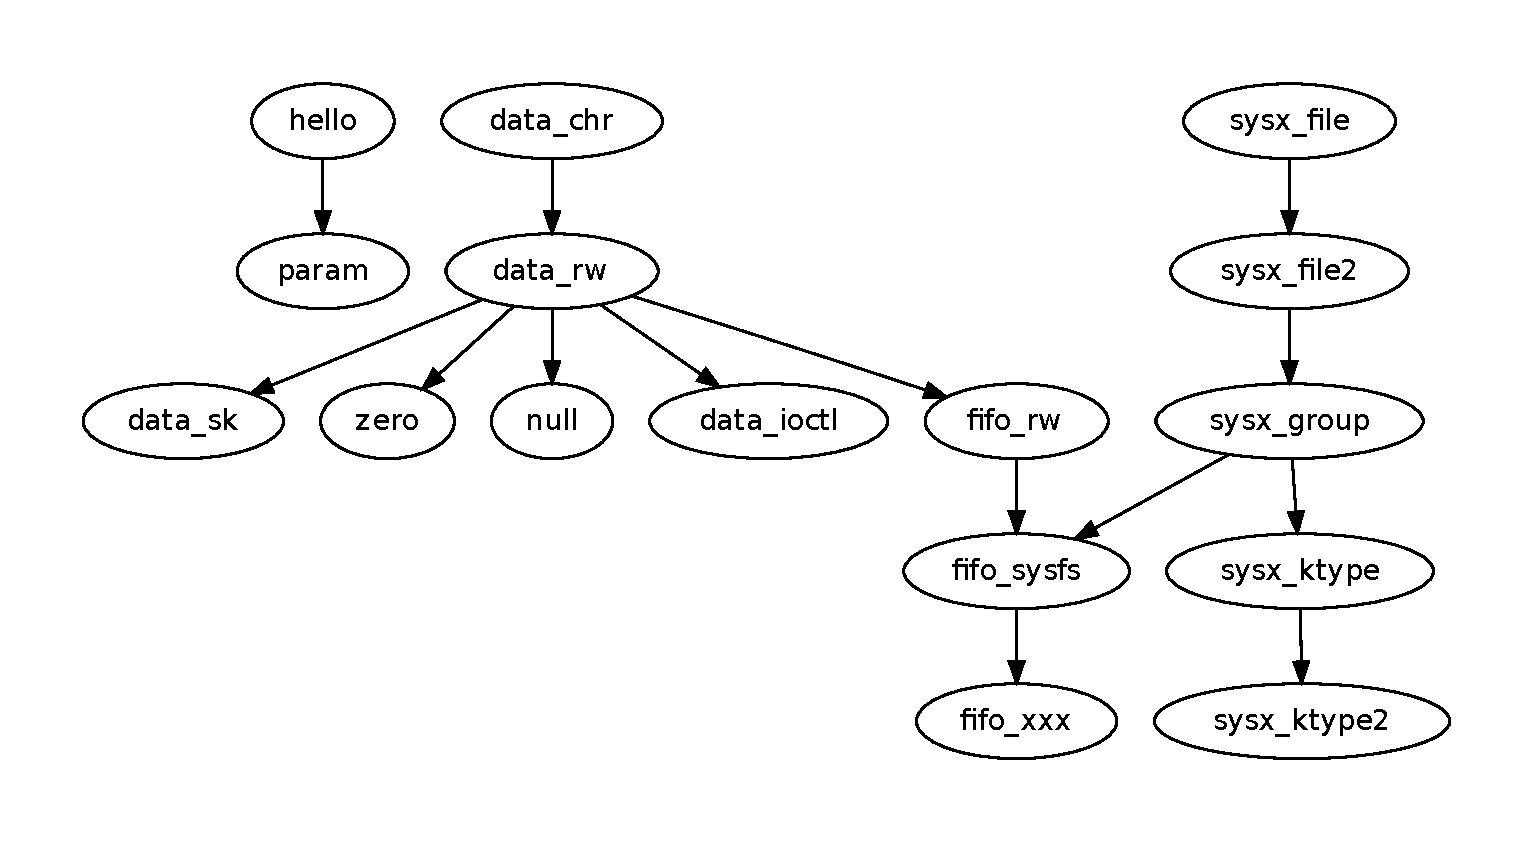
\includegraphics[scale=0.6]{hierarchy/hier}
\end{center}
\caption{Hierarch of kernel module examples.}\label{fig:hier}
\end{figure*}

% }}}

\section{Hello, World}
\subsection{hello}

The \verb+hello+ module (Listing \ref{lst:hello}) simply prints message
when it is loaded and unload.

\begin{verbatim}
hello$ make
 (should compile without error, resulting in hello.ko)
hello$ sudo insmod hello.ko
 Hello, World
hello$ sudo rmmod hello
 Goodbye, cruel world
\end{verbatim}

\lstinputlisting[float=ht,
				 caption={Hello, World module in hello/hello.c},
			 	 label={lst:hello}]
	{../hello/hello.c}

The \verb+__init+ and \verb+__exit+ on lines 4 and 10
are optional hints for the compiler.  For example in the case of
\verb+__init+ it may discard that code after initiliazation
has been completed.

The \verb+printk+ statements are the \verb+printf+ of the
kernel domain.  There are various levels, in this case
\verb+KERN_ALERT+ is used which will cause the messages
to appear on the console.  Notice that there is no comma
between the level and the message.

The \verb+MODULE_AUTHOR+ and \verb+MODULE_LICENSE+ on lines 15 and 16
are optional but recommended.  There are various other \verb+MODULE_*+
as well (\verb+linux/module.h+).

The \verb+module_init+ and \verb+module_exit+ tell the kernel which
functions to call when this module is loaded (\verb+insmod+) and
unloaded (\verb+rmmod+).

\clearpage
\subsection{param}

The \verb+param+ module expands upon the \verb+hello+ module to
take a parameter specifying how many times to print the message.

\begin{verbatim}
param$ sudo insmod hello.ko howmany=2
 Hello, World
 Hello, World
param$ sudo rmmod hello
 Goodbye, cruel world
 Goodbye, cruel world
\end{verbatim}

Listing \ref{lst:param-diff} shows the differences between this
parameterized hello world module and the previous \verb+hello+ module.

\lstinputlisting[float=ht,
				 caption={param\$ diff -u hello.c ../hello/hello.c},
			 	 label={lst:param-diff}]
	{../param/diff}

To use a parameter a global variable has been created named \verb+howmany+
on line 8.
And on line 9 the \verb+module_param+ function is used to tell
the kernel about this parameter
\footnote{The \verb+module_param+ function create a sysfs entry
in \verb+/sys/module/parameters/howmany+.  \verb+sysfs+ will
be discussed in detail in later modules.}.

On lines 13-19 and 25-30 it can be seen that the same message
is printed \verb+howmany+ times.

\section{Read/Write Data}

The \verb+data+ module allocates a memory from ram which can
be read from and written to.
This is accomplished as a character device and supports all
the usual file operations.

\subsection{data\_chr}

The first step is to construct the basic infrastructure for
a character driver as shown in Listing \ref{lst:data_chr}.

The \verb+DEVICE_NAME+ on line 8 defines the string which will
be used to define the module name in later functions.

Lines 10-17 are the global variables that will be used.
The \verb+struct data_dev+ is the per device structure.
Notice that a character device is placed inside.

The \verb+file_operations+ (line 19-21) in this case only
defines the \verb+.owner+.  Upcoming modules will and references
to the open, close, read, write, and seek functions to this structure.

The \verb+data_cleanup+ function takes care of unregistering and
removing the various that were created during \verb+data_init+.
It will be called if module initialization fails or during module
removal.  Different authors use different styles for cleanup.
It is not always done with a separate function.
Some use several goto labels each with levels of items to remove
\footnote{Recalling the \verb+__init+ directive, it might be
beneficial use the goto style since this code will be
purged after init.}.

\lstinputlisting[caption={Data driver infrastructure.},
			 	 label={lst:data_chr}]
	{../data_chr/data.c}


%\lstinputlisting[linerange=26-30,
%				firstnumber=26]{../hello/hello.c}


\subsection{data\_rw}
\subsection{data\_sk}
\subsection{ioctlx}
\subsection{null}
\subsection{zero}

\section{Sysfs}
\subsection{sysx\_file}
\subsection{sysx\_file2}
\subsection{sysx\_group}
\subsection{sysx\_ktype}
\subsection{sysx\_ktype2}

\section{Concurrency}
\subsection{fifo\_rw}
\subsection{fifo\_sysfs}
\subsection{fifo\_xxx}
\subsection{fifo\_fix}

\pagebreak
\printbibliography

%\pagebreak
%\printindex

\end{document}
